%%%%%%%%%%%%%%%%%%%%%%%%%%%%%%%%%%%%%%%%%%%%%%%%%%%%%%%%%%%%%%%%%%%%%%%%%%%
%% This file is part of the book
%%
%% Algorithmic Graph Theory
%% http://code.google.com/p/graph-theory-algorithms-book/
%%
%% Copyright (C) 2009--2011 Minh Van Nguyen <nguyenminh2@gmail.com>
%%
%% See the file COPYING for copying conditions.
%%%%%%%%%%%%%%%%%%%%%%%%%%%%%%%%%%%%%%%%%%%%%%%%%%%%%%%%%%%%%%%%%%%%%%%%%%%

\documentclass{article}

\usepackage{pgfplots}
\usepackage{subfigure}
\usetikzlibrary{external}
\tikzexternalize{distance-distribution}

\begin{document}

\begin{figure}
\subfigure[Zachary karate club network~\cite{Zachary1977}.]
{
\begin{tikzpicture}
[every mark/.append style={scale=0.5},%
 scale=0.9]
\begin{axis}[%
  enlargelimits=false%
]
\addplot+[sharp plot] coordinates
{
  (1, 0.139037433155080)  (2, 0.472370766488414)
  (3, 0.244206773618538)  (4, 0.130124777183601)
  (5, 0.0142602495543672)
};
\end{axis}
\end{tikzpicture}
}
%%
%%
\quad
\subfigure[C. elegans neural network~\cite{WattsStrogatz1998,WhiteEtAl1986}.]
{
\begin{tikzpicture}
[every mark/.append style={scale=0.5},%
 scale=0.9]
\begin{axis}[%
  enlargelimits=false%
]
\addplot+[sharp plot] coordinates
{
  (1, 0.0346667849328839)     (2, 0.173954822305009)
  (3, 0.300780557033883)      (4, 0.208932056058187)
  (5, 0.0949234226243274)     (6, 0.0639081071491928)
  (7, 0.0490509136065283)     (8, 0.0293300218792502)
  (9, 0.0213174856602212)     (10, 0.0139849801904086)
  (11, 0.00671160782922358)   (12, 0.00209922535627698)
  (13, 0.000310448820294483)  (14, 0.0000295665543137603)
};
\end{axis}
\end{tikzpicture}
}
%%
%%
\subfigure[Power grid network~\cite{WattsStrogatz1998}.]
{
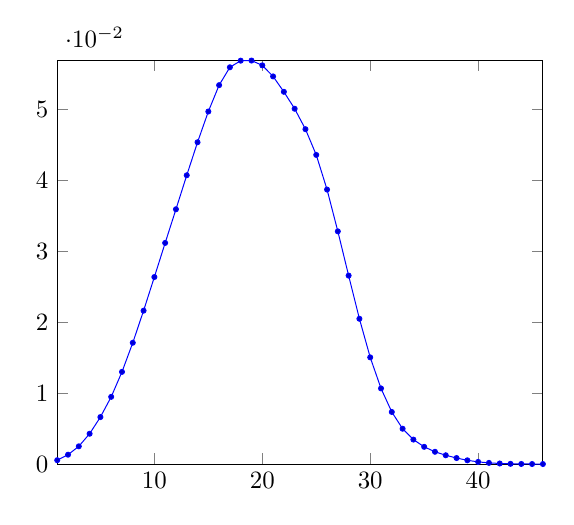
\begin{tikzpicture}
[every mark/.append style={scale=0.5},%
 scale=0.9]
\begin{axis}[%
  enlargelimits=false%
]
\addplot+[sharp plot] coordinates
{
  (1, 0.000540302697334621)    (2, 0.00131388440275412)
  (3, 0.00249879755200434)     (4, 0.00426965316237677)
  (5, 0.00661727411799313)     (6, 0.00946865318450018)
  (7, 0.0129893062018457)      (8, 0.0170914769994436)
  (9, 0.0216128453401965)      (10, 0.0263555296629786)
  (11, 0.0311600775794046)     (12, 0.0359045645499485)
  (13, 0.0406960842393687)     (14, 0.0453504388218222)
  (15, 0.0496812181310312)     (16, 0.0533967209837213)
  (17, 0.0559178058171443)     (18, 0.0568477262466334)
  (19, 0.0568661624169246)     (20, 0.0561867280877922)
  (21, 0.0546287487903824)     (22, 0.0524594260861158)
  (23, 0.0500720649412050)     (24, 0.0471905324939550)
  (25, 0.0435663091688401)     (26, 0.0386844932142603)
  (27, 0.0327940138984142)     (28, 0.0265576720279050)
  (29, 0.0204743913400802)     (30, 0.0150351475344285)
  (31, 0.0106571716292740)     (32, 0.00733562925107360)
  (33, 0.00497620914647087)    (34, 0.00344715415178458)
  (35, 0.00242570837911649)    (36, 0.00172742818701979)
  (37, 0.00123735381141191)    (38, 0.000847162509515112)
  (39, 0.000528831302486753)   (40, 0.000301369930360439)
  (41, 0.000164204823393779)   (42, 0.0000785790547079014)
  (43, 0.0000302353192775971)  (44, 0.0000106520095015925)
  (45, 3.60529552361591e-6)    (46, 6.55508277021075e-7)
};
\end{axis}
\end{tikzpicture}
}
%%
%%
\qquad
\subfigure[Condensed matter coauthorship network~\cite{Newman2001b}.]
{
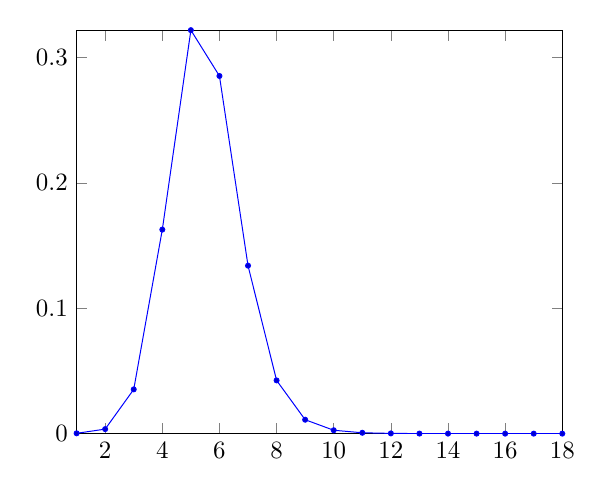
\begin{tikzpicture}
[every mark/.append style={scale=0.5},%
 scale=0.9]
\begin{axis}[%
  enlargelimits=false%
]
\addplot+[sharp plot] coordinates
{
  (1, 0.000264366917296138)    (2, 0.00361521492316542)
  (3, 0.0352921611353204)      (4, 0.162705582489662)
  (5, 0.321747496907179)       (6, 0.285209332522791)
  (7, 0.133944826388271)       (8, 0.0424488948269472)
  (9, 0.0111017102047600)      (10, 0.00270642308054925)
  (11, 0.000694119459596421)   (12, 0.000202672325160658)
  (13, 0.0000539137395725535)  (14, 0.0000109903978185300)
  (15, 1.87787739287041e-6)    (16, 3.61130267859694e-7)
  (17, 5.26648307295387e-8)    (18, 3.00941889883078e-9)
};
\end{axis}
\end{tikzpicture}
}
\end{figure}

\end{document}
